\section{Preliminaries}
\label{sec:preliminaries}

The vocabulary used throughout this document is described in the Glossary \cite{glossary} (e.g., \emph{subnets}, \emph{actors}, \emph{accounts}, \emph{users}, and \emph{\ipc agents}).
The reader is assumed to be familiar with the terminology defined there.
\jorge{Despite this note, the vocabulary seems to be defined throughout the body. If we're defining in the body anyway, the appendix seems redundant -- this isn't a book.}
\marko{If the glossary is stable, I suggest bringing it to the main body of the paper by defining concepts inline, as we go. Glossary can additionally stay in the appendix, for quick reference.}

\paragraph{Basic abstractions.}
A \emph{subnet} consists of multiple \emph{replicas}, yet we abstract a subnet as a single entity which maintains an  abstraction of \emph{replicated state} (of which each replica maintains a copy and that all replicas agree on)
that can only be modified through \emph{transactions} \gls{submit}ted either by \emph{\glspl{user}} or by an \emph{\gls{agent}}.
A sequence of transactions can be batched into a \emph{\gls{block}} to amortize the ordering overhead.
% \akosh{What about cron, and similar end-of-epoch changes? Although I saw cron will be removed from Filecoin.}
% \jorge{There are proposals to fix some cron issues (https://github.com/filecoin-project/FIPs/discussions/638),
% but I don't think the current direction is towards removing it; in fact, I think there are very strong opinions against that solution.}
% \matej{Even that must be bound to blocks. As I understand it, it is some actions triggered every k blocks.
% That can be easily modeled by every k-th block containing an (implicit) transaction triggering the action (submitted by some implicit system-level user).}
We further abstract away the concrete mechanism of transaction submission and execution, as it is specific to the implementation of each particular subnet.

For example, the replicated state of a subnet representing a game of chess would consist of the players' identities, a flag indicating which player's turn it is, and positions of the individual pieces on the board,
while players' moves would be performed by submitting transactions to the subnet.

\paragraph{Interaction between subnets.}
In \ipc, the replicated state (or, simply, state) of one subnet often needs to react to changes in the state of another subnet.
E.g., after a game hosted in a subnet finishes, the implementation of the game logic might need to update the involved players' rankings in its parent subnet based on the result of the game.
As the state of every subnet evolves independently of the state of other subnets,
\emph{IPC establishes a protocol for interaction between the states of different subnets}.

At the basis of the protocol, IPC relies on  \emph{\pofsFull (\glspl{pof})}.
In a nutshell, a \pof is data that proves that a subnet irreversibly reached a certain replicated state.
Regardless of the approach to \emph{\gls{finality}} that the  \emph{ordering protocol} of a subnet uses (e.g., immediate finality for classic BFT protocols \cite{Algorand}, or probabilistic finality in PoW-based systems \cite{nakamoto2008bitcoin}),
a \pof serves to convince the verifier that the replicated state the \pof refers to will not be rolled back. This helps IPC establish the partial ordering between the states of two subnets. 


For example, for a subnet using a BFT-style ordering protocol, a quorum of signatures produced by its replicas can constitute a \pof.
To prove the finality of the state of a subnet based on a longest-chain-style protocol,
a \pof might consist of signatures of a committee of processes considering the state deep enough (for some parametrized notion of ``deep enough'') in the chain.
This committee can be, for example, a quorum of replicas of the very subnet that is to verify the \pof.
If the verifying subnet itself is a longest-chain one, a \pof can be as simple as a hash of the proving subnet's block,
with every replica of the verifying subnet deciding locally about the \pof's validity (potentially leading to forks in the worst case).

If a \pof is associated with subnet \subnetName{A}'s replicated state at \emph{\gls{block height}} $h_\subnetName{A}$,
and the \pof is included in subnet \subnetName{B}'s replicated state at block height $h_\subnetName{B}$,
then subnet \subnetName{B}'s replicated logic will consider all \subnetName{A}'s state changes up to $h_\subnetName{A}$
to have occurred at \subnetName{B}'s height $h_\subnetName{B}$.
(Unless, of course, another \pof' of $h'_\subnetName{A}$ has been included by \subnetName{B} at $h'_\subnetName{B}$,
in which case \subnetName{B} consideres only the state changes between $h'_\subnetName{A}$ and $h_\subnetName{A}$ to have occured at $h_\subnetName{B}$).

In the following, for some representation of a subnet's replicated state (e.g., its full serialization or a handle that can be used to retrieve it in a content-addressable way, such as an IPFS content identifier (CID)),
we denote by {\pof}($state$) the proof that a subnet reached $state$.
%
% \marko{but what if it is - esp at longest chain parent net?}
% \arp{what happens if state is rolled back before a checkpoint for example?. If we are talking about payments, if checkpoint occurred and then state rolled back then whoever got its money back (due to the rollback) cannot withdraw that money to the parent anymore. If we are talking about state then behavior is undefined.}
% \matej{If the state is rolled back despite a \pof, then the assumptions underlying the verification of the \pof were wrong and the verifier treats the subnet as faulty (e.g. the same way as if the adversary started controlling the majority of its replicas / conputing poser / stake ...)}
% \akosh{There's always that word "assume"... perhaps what's missing from the defintion of PoF is that violations are detectable, e.g. by checkpointing.}
% \matej{Are they though in all the imaginable cases? I'm not quite sure. I assume that by ``violation'' you mean a state with a valid \pof being rolled back. Is that the case?}
% \jorge{I think I +1 Akosh on "assume". If we're saying a rollback is a violation, then this isn't a question of assumptions -- it's a question of definition. Something like "... proof that a subnet reached $state$ and cannot be rolled back without triggering a violation."?}.
% \matej{I just removed the second part of the sentence to avoid this confusion. It's quite clear from the definition of a \pof (it "convinces the verifier that the state will not be rolled back") and removes the necessity of any kind of assumptions. I.e., only the verifier locally makes whatever assumptions they need to be reasonably "convinced" by the \pof.}
We also denote by {\pof}(\tx{tx}) the proof that a subnet reached a state in which transaction \tx{tx} already has been applied to the replicated state.

\paragraph{Naming subnets.}
We assign each subnet a name that is unique among all the children of the same parent.
Similarly to the notation used in a file system, the name of a child subnet is always prefixed by the name of its parent.
For example, subnets \subnetName{P/C} and \subnetName{P/D} would both be children of subnet \subnetName{P}.

\paragraph{Representing value.}
For each pair of subnets in a parent-child relationship, we assume that there exists a notion of \emph{value} (measured in \emph{\glspl{coin}}) common to both subnets.%
\footnote{One can easily generalize the design to decouple the use of value between a parent and its child, but we stick with using the same kind of value in both subnets for simplicity.}
We represent this value by associating some number of coins (also referred to as funds) with \glspl{account} and actors in a subnet's replicated state.
The number of coins associated with an account is the account's \emph{\gls{balance}}.
Each user is assumed to have an account in each subnet the user interacts with.
All the transactions spending coins from an account must be signed by the corresponding user's private key.
For ease of presentation, we do not explicitly include these signatures in the further description of \ipc.

We also assume that the submission, ordering, and application of transactions is associated with a cost (known as transaction fees, or \emph{gas}).
Each \gls{subnet client} (user \gls{wallet} or IPC agent) submitting a transaction to a subnet must have an account in that subnet, from which this cost is deducted.
If the funds are insufficient, the subnet may fail to execute the transaction.

Note that the operation of \ipc requires the submission and processing of transactions that are not easily attributed to a concrete user.
This is the case with transactions that an \ipc agent submits on behalf of a whole subnet.
% We discuss incentivization of participants to run \ipc agents and pay for the associated transaction fees in \Cref{sec:refunds-rewards}.
\matej{Move this part after \ipc agent and actors, as it already uses those terms. On the other hand, it would be nice to have it before the trust model. Maybe we could move the trust model to be last...}

\paragraph{Notation.} We refer to an account \accountName{a} in the replicated state of subnet \subnetName{S} as \subnetName{S}.\accountName{a}.
To denote a function of an actor in the replicated state of a subnet, we write \funcNameFull{Subnet}{Actor}{Function}.
E.g., the \emph{IPC Gateway Actor} (\gw) function \funcName{CreateChild} in subnet \subnetName{P} is denoted \funcNameFull{P}{\gw}{CreateChild}.
We also use this notation for a transaction \tx{tx} submitted to subnet \subnetName{P} that invokes the function, e.g., \tx{tx} = \funcNameFull{P}{\gw}{CreateChild}$(\subnetName{P/C}, params)$.

\paragraph{Trust model.}

\ipc can be deployed in an adversarial environment, where some participants might be malicious (Byzantine) and actively try to subvert the system.
For each subnet, the assumptions under which the subnet's implementation is guaranteed to operate correctly may differ.
While some may rely on honest participants controlling a certain fraction of the overall involved resource such as computing power, storage capacity, or staked collateral,
others may depend on a simple majority of honest replicas.
In case of a violation of these assumptions, there are no guarantees about the replicated state of the affected subnet.
The users of a subnet must bear this risk and choose the subnets to use accordingly.

\ipc as a system is based on two fundamental principles:
\begin{enumerate}
    
    \item \emph{Hierarchical trust}: Whatever is part of the replicated state of a subnet is considered a ground truth by all children of that subnet.
    For example, if a child subnet's membership (i.e., set of replicas) is maintained in the state of its parent (as is the case for \ipc-native PoS-based subnets, see \Cref{sec:pos-subnets}),
    long-range attacks within the child subnet can be easily ruled out. If a parent subnet fails as a whole, there are no guarantees about the correct behavior of its children. However, if the parent stops being available, the child subnet can continue to work, albeit disconnected from the rest of the IPC hierarchy until the parent becomes available.

    \item \emph{Subnet firewall property}: In case a whole subnet fails (e.g., if the underlying assumptions made by the protocol it is based on are violated),
    at most as many coins can be impacted by the failure (e.g., double-spent or permanently lost) as have been deposited to the subnet from its parent.
    That is, a user is able to manage the risk of using a potentially non-robust subnet through the amount of funds they deposit and/or accept to receive in it.
    % \guy{I suggest to describe it in terms of parent-child for better clarity. E.g., start with the sentence ``A failure at a child subnet has a limited effect on its parent subnet. The effect is limited to the amount of tokens that are deposited from the parent into the child." }
\end{enumerate}

The above principles enable child subnets to ``inherit'' some of their parents' robustness through \emph{checkpointing},
where a child subnet regularly includes its replicated state (or a reference to it) in its parent's replicated state.
In case the child subnet fails, there exists a record of the evolution of its state in the parent.
This enables participants (e.g., former users of the failed subnet) to agree on picking up an older version of the child subnet's state from before the occurrence of the failure
and, say, use that version as the initial state of a new, more robust subnet.

We envision subnets higher up in the hierarchy to be more robust than their descendants, in the sense that it should be harder / less probable to violate the assumptions their correctness is based on.
For example, a robust public system such as Filecoin, backed by a substantial amount of resources, can serve as a the rootnet,
while its descendant subnets, where less is at stake in case of a failure of the whole subnet, can more easily sacrifice a part of their robustness, e.g., for the sake of performance.


\paragraph{\ipc actors.}
For inter-subnet communication, \ipc relies on two special types of actors: the \gwFull (\gw) and the \saFull (\sa).
In a nutshell, their functions are as follows.
\begin{enumerate}
    \item The \gw is an actor that contains all \ipc-related information and logic associated with a subnet that needs to be replicated \emph{in the subnet itself}.
    Each subnet contains exactly one \gw. We describe the \gw in detail in \Cref{sec:gw}
    % \marko{Why is IGA an actor an not a blob of information? When does the state of IGA need to change (to demonstrate the need of IGA to be an actor) and how does it change (governance)?}
    % \matej{Those questions should be answered in \Cref{sec:gw}}

    \item The \sa is the \gw's parent-side counterpart, i.e., it is an actor in a parent subnet's replicated state,
    containing all the data and logic associated with a particular child subnet -- we say the \sa ``governs'' that child subnet.
    A subnet contains as many \saFulls as the number of its children.
    We refer to the \sa governing child subnet \subnetName{C} as \saOf{C}.
    We describe the \sa in detail in \Cref{sec:sa}.

\end{enumerate}

\paragraph{\ipc agent.}

The \ipc agent is a \gls{process} that mediates the communication between a parent and a child.
It has access to the replicated states of both subnets and acts as a client of both subnets.
When the replicated state of subnet \subnetName{A} indicates the need to communicate with subnet \subnetName{B},
the \ipc agent constructs a \pof for \subnetName{A}'s replicated state and submits it as a transaction to \subnetName{B}.

\ipc does not prescribe who must run an \ipc agent, nor how the \pof is to be constructed, nor which \ipc agent must submit the transaction with the \pof.
All this is specific to the implementation of the subnets involved.
The \ipc agents may run a protocol for choosing which of them submit(s) the transaction, or even resort to a simplistic approach where each \ipc agent submits an identical transaction.
In our reference implementation (\cref{sec:ref-impl}), for example, we construct the \pof directly in the verifying subnet's (\subnetName{B}'s) replicated state,
using one \ipc agent per replica of the proving subnet (\subnetName{A}).
When describing the functionality of \ipc and referring to ``the \ipc agent'' submitting a \pof,
we assume such a subnet-specific mechanism for choosing one (or multiple) \ipc agent(s) to perform the actual submission.

The interaction between subnets through \ipc agents is depicted in \cref{fig:interfaces}.

\begin{figure}[ht]
     \centering
     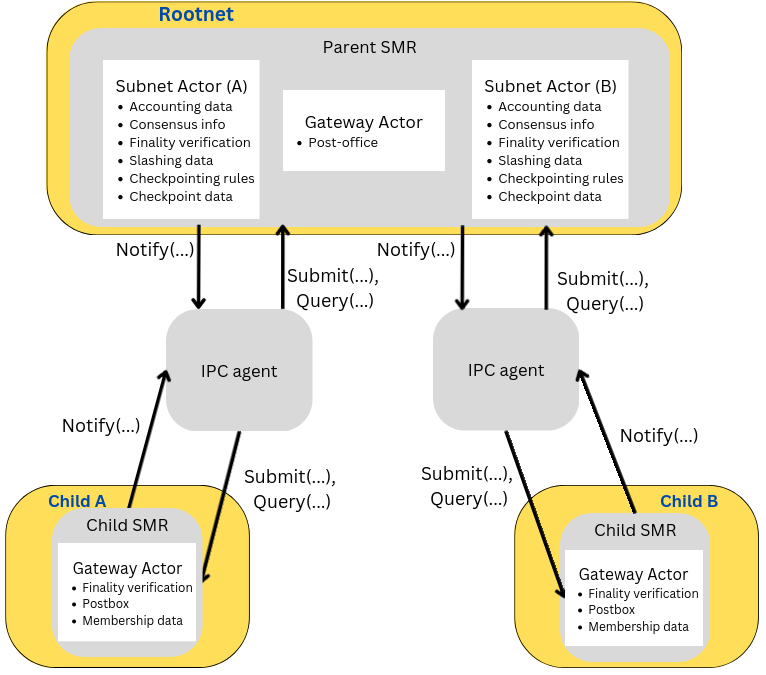
\includegraphics[width=0.75\textwidth]{compsintf-2subnets}
     \caption{The basic \ipc components and their interfaces in an example with one parent and 2 child subnets (A and B).}
     \label{fig:interfaces}
 \end{figure}


\paragraph{Incentives.}

In general, submitting transactions (and their subsequent execution by the subnet) is associated with a \emph{cost} (often referred to as ``gas").
We refer to the cost associated with a transaction as the \emph{transaction fee}, measured in coins.
A participant running an IPC agent is not necessarily interested in participating in such a costly protocol without incentives.
Moreover, the replicas of a subnet might need to cooperate with IPC agents during the construction of \pofsFull.
Even though certain deviations from the protocol can be detected and penalized (see \Cref{sec:slash}),
participants running subnet replicas might also need positive incentives to participate in the creation of a \pof.

The key to providing incentives for \ipc agents and replicas is that the \sa and the \gw can,
as actors, hold funds that their logic can distribute among other accounts or actors on their respective subnets.
Thus, the actors can be configured to reimburse an account associated with the \ipc agent submitting a transaction (potentially adding an extra reward), as well as to reward or penalize accounts.

The source of funding for the \gw and / or \sa is subnet-specific.
For example, a subnet’s implementation can require a certain part of each transaction fee to be sent to the subnet's \gw.
An \sa can be funded, for example, through transfers (withdrawals) of funds from the child subnet, or by charging fees for propagating cross-net transactions.

To incentivize the replicas of a subnet to collaborate with an IPC agent on the creation of \pofsFull, a similar mechanism can be deployed.
For example, a valid \pof would include metadata, where the replicas that participated in its creation could insert an address to receive a reward when the \pof is accepted.

\begin{example}
Our gaming platform from \Cref{sec:example-use-case} could use the following approach.
Each replica of the \subnetName{L2} subnet running the gaming platform is registered in the \gw of the subnet itself and has an associated account controlled by the participant operating the replica.
(Such a participant could be, for example, a local club of players who bought a server and are paying for internet connection.)
The \subnetName{L2} subnet is configured to pay a small fee to the \gw for each transaction executed by the subnet.
The \gw periodically (e.g., every 1000 blocks) re-distributes a part of the collected fees to the accounts associated with the replicas.

Each participant also controls an account in the rootnet (\subnetName{L1}) and operates an \ipc agent (e.g., running on the same machine as the replica)
to mediate the interactions between \subnetName{L1} and \subnetName{L2} (e.g., periodic checkpointing of \subnetName{L1}'s state to \subnetName{L2}).
The definition of \saOf{L2} requires a valid \pof to contain a withdrawal transaction transferring a certain amount of funds (e.g., from the \gw in \subnetName{L2})
to the \subnetName{L1} account associated with the \ipc agent submitting the \pof.
This way, the participant operating the \ipc agent has an incentive to submit the \pof.
To prevent too many or repeated submissions, the \saOf{L2} adjusts the reward based on the most recent \pof already submitted.

\end{example}

% \TODO{Add example of gaming system incentives: The replicas and \ipc agents running the \subnetName{L2} subnet might get a commission from transaction fees,
% while the single-game subnets might not need explicit incentivization at all, as they are mostly run by players, whose incentive is being able to play the game.}
